\documentclass[UTF8,12pt]{article} % 12pt 为字号大小
\usepackage{amssymb,amsfonts,amsthm}
%\usepackage{fontspec,xltxtra,xunicode}
%\usepackage{times}
\usepackage{amsmath,bm}
\usepackage{mdwlist}
\usepackage[colorlinks,linkcolor=blue]{hyperref}
\usepackage{cleveref}

%----------
% 定义中文环境
%----------

\usepackage{xeCJK}
\usepackage{float}
\setCJKmainfont[BoldFont={Heiti SC Light},ItalicFont={Kaiti SC Regular}]{Songti SC Regular}
\setCJKsansfont{Heiti SC Light}
\setCJKfamilyfont{song}{Songti SC Regular}
\setCJKfamilyfont{zhhei}{Heiti SC Light}
\setCJKfamilyfont{zhkai}{Kaiti SC Regular}
\setCJKfamilyfont{zhfs}{STFangsong}
\setCJKfamilyfont{zhli}{Libian SC Regular}
\setCJKfamilyfont{zhyou}{Yuanti SC Regular}

\newcommand*{\songti}{\CJKfamily{zhsong}} % 宋体
\newcommand*{\heiti}{\CJKfamily{zhhei}}   % 黑体
\newcommand*{\kaiti}{\CJKfamily{zhkai}}  % 楷体
\newcommand*{\fangsong}{\CJKfamily{zhfs}} % 仿宋
\newcommand*{\lishu}{\CJKfamily{zhli}}    % 隶书
\newcommand*{\yuanti}{\CJKfamily{zhyou}} % 圆体

%----------
% 版面设置
%----------
%首段缩进
\usepackage{indentfirst}
\setlength{\parindent}{2em}

%行距
\renewcommand{\baselinestretch}{1.5} % 1.5倍行距

%页边距
\usepackage[a4paper]{geometry}
\geometry{verbose,
  tmargin=2cm,% 上边距
  bmargin=2cm,% 下边距
  lmargin=2.5cm,% 左边距
  rmargin=2.5cm % 右边距
}


%----------
% 其他宏包
%----------
%图形相关
\usepackage[x11names]{xcolor} % must before tikz, x11names defines RoyalBlue3
\usepackage{graphicx}
\graphicspath{{figures/}}
\usepackage{pstricks,pst-plot,pst-eps}
\usepackage{subfig}
\def\pgfsysdriver{pgfsys-dvipdfmx.def} % put before tikz
\usepackage{tikz}

%原文照排
\usepackage{verbatim}

%网址
\usepackage{url}

%----------
% 定理、习题与解答环境
%----------
%定理环境
\usepackage[most]{tcolorbox}
\newtcbtheorem[number within=section]{theorem}{定理}{
     enhanced,
     breakable,
     sharp corners,
     attach boxed title to top left={
       yshifttext=-1mm
     },
     colback=white,
     colframe=blue!75!black,
     fonttitle=\bfseries,
     boxed title style={
       sharp corners,
       size=small,
       colback=blue!75!black,
       colframe=blue!75!black,
     } 
}{theorem}

\newtcbtheorem[number within=section]{definition}{定义}{
     enhanced,
     breakable,
     sharp corners,
     attach boxed title to top left={
       yshifttext=-1mm
     },
     colback=white,
     colframe=blue!75!black,
     fonttitle=\bfseries,
     boxed title style={
       sharp corners,
       size=small,
       colback=blue!75!black,
       colframe=blue!75!black,
     } 
}{definition}

\newtcbtheorem[number within=section]{corollary}{推论}{
     enhanced,
     breakable,
     sharp corners,
     attach boxed title to top left={
       yshifttext=-1mm
     },
     colback=white,
     colframe=blue!75!black,
     fonttitle=\bfseries,
     boxed title style={
       sharp corners,
       size=small,
       colback=blue!75!black,
       colframe=blue!75!black,
     } 
}{corollary}

\newtcbtheorem[number within=section]{myboxes}{盒子}{
     enhanced,
     breakable,
     sharp corners,
     attach boxed title to top left={
       yshifttext=-1mm
     },
     %colback=white,
     colframe=black!75!white,
     fonttitle=\bfseries,
     boxed title style={
       sharp corners,
       size=small,
       colback=black!75!white,
       colframe=black!75!white,
     } 
}{myboxes}

%习题环境
\newtcbtheorem[]{exercise}{题}{
     enhanced,
     breakable,
     sharp corners,
     attach boxed title to top left={
       yshifttext=-1mm
     },
     colback=white,
     colframe=black,
     fonttitle=\bfseries,
     boxed title style={
       sharp corners,
       size=small,
       colback=black,
       colframe=black,
     } 
}{Problem}

%解答环境
\ifx\proof\undefined\
\newenvironment{proof}[1][\protect\proofname]{\par
\normalfont\topsep6\p@\@plus6\p@\relax
\trivlist
\itemindent\parindent
\item[\hskip\labelsep
\scshape
#1]\ignorespaces
}{%
\endtrivlist\@endpefalse
}
\fi

\renewcommand{\proofname}{\it{Solution}}

%----------
%示例:
%\begin{exs} \end{exs}
%\begin{proof}[] \end{proof}
%\begin{thm}{}{} \end{thm}
%----------

%----------
%插入图片
%\begin{figure}[htbp]
%\centering
%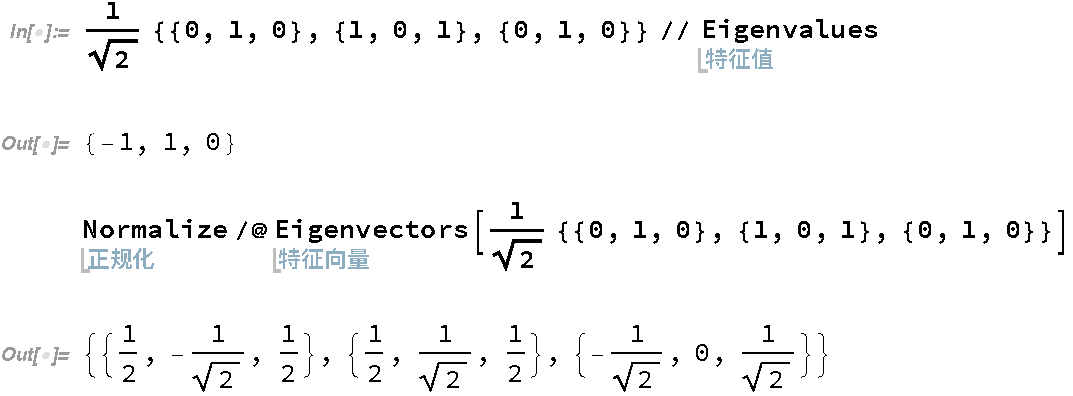
\includegraphics[width=10cm]{eigen}
%\end{figure}
%----------

%==========
% 正文部分
%==========

\begin{document}

\title{作业 06}
\author{陈昱全~SA18234049}
\date{} % 若不需要自动插入日期,则去掉前面的注释;{ } 中也可以自定义日期格式
\maketitle

\begin{exercise}{}{}
Prove $e^{-i\omega t\hat{\sigma}_{x}}=cos\omega tI-isin\omega t\hat{\sigma}_{x}$
\end{exercise}

\begin{proof}[解]
因为
\begin{align}
\hat{\sigma}_x = \begin{pmatrix}0 & 1 \\ 1 & 0\end{pmatrix} = 1\cdot\frac{1}{\sqrt{2}}\begin{pmatrix}1\\1\end{pmatrix}\cdot\frac{1}{\sqrt{2}}\begin{pmatrix}1&1\end{pmatrix} + (-1)\cdot\frac{1}{\sqrt{2}}\begin{pmatrix}-1\\1\end{pmatrix}\cdot\frac{1}{\sqrt{2}}\begin{pmatrix}-1&1\end{pmatrix}
\end{align}
所以
\begin{align}
e^{-i\omega t\hat{\sigma}_x} &= e^{-i\omega t}\frac{1}{\sqrt{2}}\begin{pmatrix}1\\1\end{pmatrix}\cdot\frac{1}{\sqrt{2}}\begin{pmatrix}1&1\end{pmatrix} + e^{i\omega t}\frac{1}{\sqrt{2}}\begin{pmatrix}-1\\1\end{pmatrix}\cdot\frac{1}{\sqrt{2}}\begin{pmatrix}-1&1\end{pmatrix}\notag\\
&= cos\omega tI-isin\omega t\hat{\sigma}_{x}
\end{align}
也可以用上课时说的 $\begin{cases}e^A = I + A + \frac{A^2}{2!} + ...\\ \sigma_x^2 = I\end{cases}$ 来化简,这两种方式等效。
\end{proof}

\begin{exercise}{}{}
Detuned Rabi flopping for a spin-1/2 particle with energy spacing $\omega_0$ apply an oscillating magnetic with frequency $\omega_0+\delta$, and Rabi rate $\Omega$, so we have $H(t) = \hbar\frac{\omega_0}{2}\sigma_{z} + \hbar\Omega\sigma_{x}cos((\omega+\delta)t)$\\
(1) Choose a proper transformation and apply rotating wave approximation to make $H(t)$ time-independent, so that $H_{int}=-\hbar\frac{\delta}{2}\sigma_z+\hbar\frac{\Omega}{2}\sigma_x$\\
(2) Solve for eigenvalue $\lambda_+,\lambda_-$ and eigenstate $|\psi_+\rangle,|\psi_-\rangle$ for $H_{int}$ in the basis of $\sigma_z~\{|0\rangle,|1\rangle\}$\\
(3) With $|\psi(t=0)\rangle=|\psi_0\rangle=\begin{pmatrix} 1 \\0 \end{pmatrix}$ solve for the overlap between $|\psi_0\rangle$ and $|\psi(t)\rangle$, defined as $|\langle\psi_0|\psi(t)\rangle|^2$. Hint: use $|\psi(t)\rangle=e^{-\frac{i}{\hbar}Ht}|\psi(0)\rangle$, and $H=\lambda_+|\psi_+\rangle\langle\psi_+|+\lambda_-|\psi_-\rangle\langle\psi_-|$. We can assume $\Omega$ is real for simplicity.
\end{exercise}

\begin{proof}[解]~\par
(1)暂时没弄懂课堂上这步的化简
\begin{figure}[H]
\begin{center}
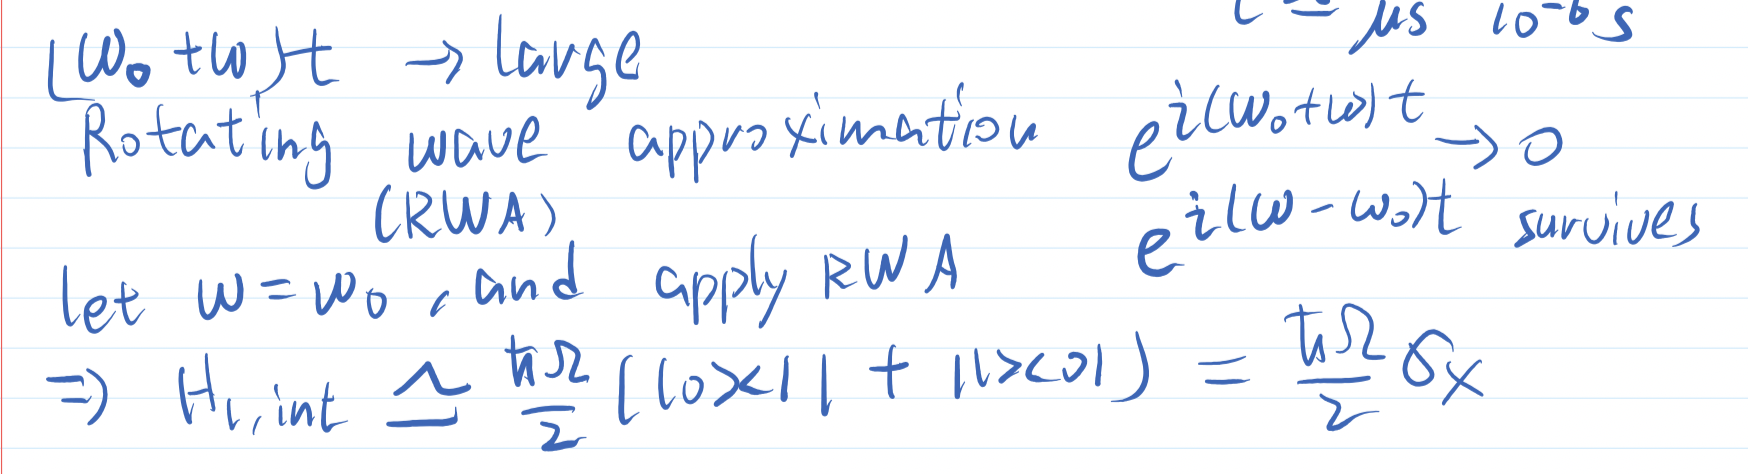
\includegraphics[width=10cm]{hint}
%\caption{}
%\label{}
\end{center}
\end{figure}
体系的哈密顿量
\begin{align}
H(t) &= \hbar\frac{\omega_0}{2}\sigma_{z} + \hbar\Omega\sigma_{x}cos((\omega+\delta)t) \notag\\
&= \hbar\frac{\omega_0 + \delta}{2}\sigma_{z} + \left(\hbar\Omega\sigma_{x}cos((\omega+\delta)t) - \hbar\frac{\delta}{2}\sigma_z\right)
\end{align}
令$H_0 = \hbar\frac{\omega_0 + \delta}{2}\sigma_{z},~H_1 = \hbar\Omega\sigma_{x}cos((\omega+\delta)t) - \hbar\frac{\delta}{2}\sigma_z$,则
\begin{align}
H_{int} = e^{\frac{i}{\hbar}H_0t} H_1 e^{-\frac{i}{\hbar}H_0t}
\end{align}
\par(2)现在已知$H_{int}=-\hbar\frac{\delta}{2}\sigma_z+\hbar\frac{\Omega}{2}\sigma_x$,我们求解它的本征值和本征态:
\begin{figure}[H]
\begin{center}
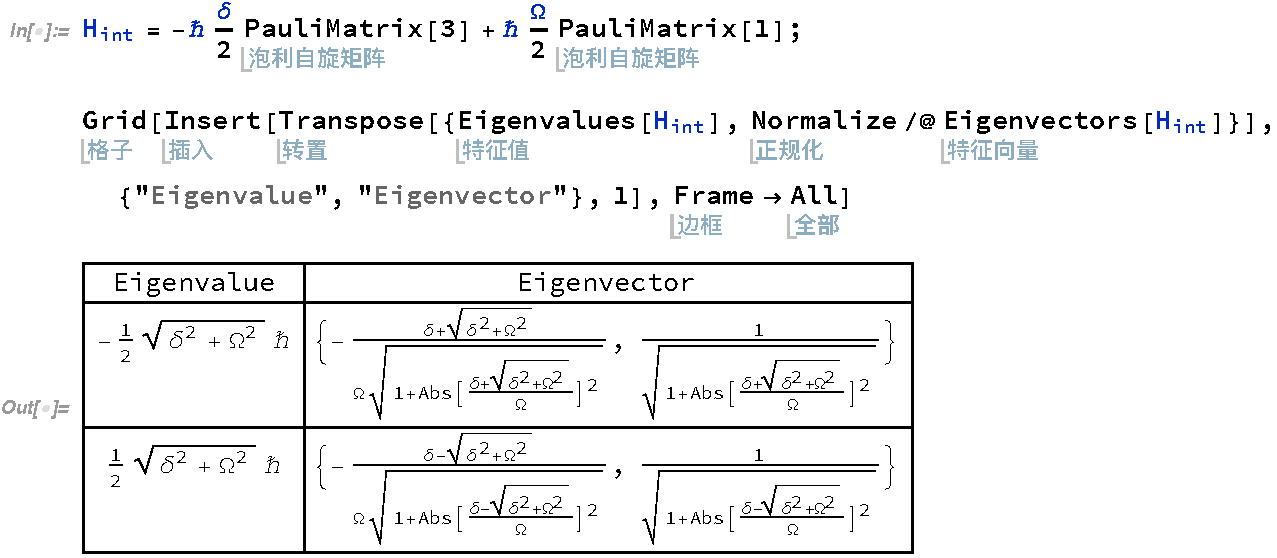
\includegraphics[width=14cm]{eigencal}
%\caption{}
%\label{}
\end{center}
\end{figure}
(3)已知$|\psi(0)\rangle = \begin{pmatrix}1\\0\end{pmatrix}$,
\begin{align}
e^{-\frac{i}{\hbar}Ht} = e^{-\frac{i}{\hbar}\lambda_+t}|\psi_+\rangle\langle\psi_+| + e^{-\frac{i}{\hbar}\lambda_-t}|\psi_-\rangle\langle\psi_-|
\end{align}
所以
\begin{align}
|\psi(t)\rangle = e^{-\frac{i}{\hbar}Ht}|\psi(0)\rangle = e^{-\frac{i}{\hbar}\lambda_+t}|\psi_+\rangle\langle\psi_+|0\rangle + e^{-\frac{i}{\hbar}\lambda_-t}|\psi_-\rangle\langle\psi_-|0\rangle
\end{align}
左乘$\langle\psi(0)|$,
\begin{align}
\langle\psi(0)|\psi(t)\rangle &= e^{-\frac{i}{\hbar}\lambda_+t}\langle0|\psi_+\rangle\langle\psi_+|0\rangle + e^{-\frac{i}{\hbar}\lambda_-t}\langle0|\psi_-\rangle\langle\psi_-|0\rangle \notag\\
&= e^{-\frac{i}{\hbar}\lambda_+t}|\langle0|\psi_+\rangle|^2 + e^{-\frac{i}{\hbar}\lambda_-t}|\langle0|\psi_-\rangle|^2
\end{align}
令$\{\delta,\Omega\}\in\mathbb{R}$,可以求出overlap
\begin{align}
|\langle\psi(0)|\psi(t)\rangle|^2 = \frac{2 \delta ^2+\Omega ^2 \cos \left(t \sqrt{\delta ^2+\Omega ^2}\right)+\Omega ^2}{2 \left(\delta ^2+\Omega ^2\right)}
\end{align} 
\end{proof}

\begin{exercise}{}{}
Proof $Tr(\rho^2)=1$ correspond to $\rho=|\psi\rangle\langle\psi|$, a pure state.
\end{exercise}

\begin{proof}[解]
假设$\rho = \sum_{i}p_i|\psi_i\rangle\langle\psi_i|$为一般的混态,我们求解它的$Tr(\rho^2)$。
\begin{align}
\rho^2 = \left(\sum_{i}p_i|\psi_i\rangle\langle\psi_i|\right)\left(\sum_{j}p_j|\psi_j\rangle\langle\psi_j|\right)
\end{align}
选取一组正交归一基$\{|n\rangle\}$,每个态$|\psi_i\rangle$可以在这组基下展开为
\begin{align}
|\psi_i\rangle = \sum_n a_{in}|n\rangle
\end{align}
则
\begin{align}
\rho = \sum_{i,n,n'} p_i a_{in} a^*_{in'} |n\rangle\langle n'|
\end{align}
$\rho^2$可以展开为
\begin{align}
\rho^2 &= \left(\sum_{i,n,n'} p_i a_{in} a^*_{in'} |n\rangle\langle n'|\right)\left(\sum_{j,m,m'} p_j a_{jm} a^*_{jkm'} |m\rangle\langle m'|\right) \notag\\
&= \sum_{i,n,n',j,m,m'} p_i p_j a_{in} a^*_{in'} a_{jm} a^*_{jm'} |n\rangle\langle n'|m\rangle\langle m'| \notag\\
&= \sum_{i,j,n,m,m'} p_i p_j a_{in} a^*_{im} a_{jm} a^*_{jm'} |n\rangle\langle m'|
\end{align}
则
\begin{align}
Tr(\rho^2) &= \sum_{i,j,k,n,m,m'} p_i p_j a_{in} a^*_{im} a_{jm} a^*_{jm'} \langle k|n\rangle\langle m'|k\rangle \notag\\
&= \sum_{i,j,k,m} p_i p_j \left(a_{ik} a^*_{jk}\right) \left(a^*_{im} a_{jm}\right)  \notag\\
&= \sum_{ij}p_ip_j \langle\psi_j|\psi_i\rangle\langle\psi_i|\psi_j\rangle \notag\\
&= \sum_{ij}p_ip_j |\langle\psi_i|\psi_j\rangle|^2 \\
&\le \sum_{ij}p_ip_j = 1
\end{align}
当且仅当对$\forall i,j,|\psi_i\rangle = |\psi_j\rangle$时等号成立。此时
\begin{align}
\rho = \sum_{i}p_i|\psi_i\rangle\langle\psi_i| = |\psi\rangle\langle\psi|
\end{align}
为纯态的密度矩阵。
\end{proof}

\end{document}